\let\negmedspace\undefined
\let\negthickspace\undefined
\documentclass[journal]{IEEEtran}
\usepackage[a5paper, margin=10mm, onecolumn]{geometry}
\usepackage{lmodern} % Ensure lmodern is loaded for pdflatex
\usepackage{tfrupee} % Include tfrupee package

\setlength{\headheight}{1cm} % Set the height of the header box
\setlength{\headsep}{0mm}     % Set the distance between the header box and the top of the text

\usepackage{gvv-book}
\usepackage{gvv}
\usepackage{cite}
\usepackage{amsmath,amssymb,amsfonts,amsthm}
\usepackage{algorithmic}
\usepackage{graphicx}
\usepackage{textcomp}
\usepackage{xcolor}
\usepackage{txfonts}
\usepackage{listings}
\usepackage{enumitem}
\usepackage{mathtools}
\usepackage{gensymb}
\usepackage{comment}
\usepackage[breaklinks=true]{hyperref}
\usepackage{tkz-euclide} 
\usepackage{listings}
\usepackage{gvv}                                        
\def\inputGnumericTable{}                                 
\usepackage[latin1]{inputenc}                                
\usepackage{color}                                            
\usepackage{array}                                            
\usepackage{longtable}                                       
\usepackage{calc}                                             
\usepackage{multirow}                                         
\usepackage{hhline}                                           
\usepackage{ifthen}                                           
\usepackage{lscape}
\begin{document}

\bibliographystyle{IEEEtran}
\vspace{3cm}

\title{11.16.2.3}
\author{EE24BTECH11060-Sruthi Bijili}
% \maketitle
% \newpage
% \bigskip
{\let\newpage\relax\maketitle}
\textbf{Question:}\\
An experiment involves rolling a pair of dice and recording the numbers that come up.Describe the following events:\\
A:the sum is greater than $8$\\
B:2 occurs on either die\\
C:the sum is atleast $7$ and a multiple of $3$\\
Which pairs of these events are mutually exclusive?\\
\textbf{Solution:}\\
Let $X_1,X_2$ be the random variables taking values from 1 to 6 with probability $\frac{1}{6}$\\
THe PMF of RV $X_1$ is defined as,
   \begin{align}
  p_X\brak{X_1} = \begin{cases}
    0 & x \textless 0\\
    \frac{1}{6} &  1\leq x \leq 6\\
    0 & x \textgreater 6
  \end{cases}
\end{align}
\begin{align}
    A:X_1+X_2 \textgreater 8\\
    B:X_1=2 \textbf{ or }X_2=2\\
    C:X_1+X_2 \geq 7 ,\brak{X_1+X_2 }\% 3=0 
\end{align}
For A and B
\begin{align}
    X_1+X_2 \textgreater 8\\
    \textbf{at } X_2=2\implies X_1+2 \textgreater 8\\
    \implies X_1 \textgreater 6\\
    \implies P_{X1}\brak{x \textgreater 6}=0\\
    P\brak{AB}=0 
\end{align}
Therefore,they are mutually exclusive.\\
For B and C
\begin{align}
    X_1+X_2 \geq 7\\
    \textbf{ at }  X_2=2\\
    X_1+2\geq 7\\ 
    \implies X_1\geq 5 \\
    Y=\brak{X_1+X_2}|\brak{\brak{X_1 \geq 5}\cap \brak{X_1+X_2 }\% 3=0} 
\end{align}
\begin{align}
  p_Y\brak{X_1} = \begin{cases}
   0 & X_1=5\\
   0 & X_1=6
  \end{cases}
\end{align}
therefore,P\brak{BC}=0\\
$\implies$ $B$ and $C$ are mutually exclusive\\
For A and C 
\begin{align}
X=X_1+X_2
\end{align}
\begin{align}
p_X(x) =
\begin{cases}
\frac{x-1}{36}, & 2 \leq x \leq 7 \\
\frac{13 - x}{36}, & 8 \leq x \leq 12 \\
0, & \text{otherwise}
\end{cases}
\end{align}
Let $Y=\brak{X_1+X_2}|\brak{X_1+X_2\textgreater8 \cap \brak{X_1+X_2}\%3=0}$
\begin{align}
p_Y(X) =
\begin{cases}
\frac{1}{9}, & \text{if } X_1 + X_2 = 9 \\
\frac{1}{36}, & \text{if } X_1 + X_2 = 12 \\
0, & \text{otherwise}
\end{cases}
\end{align}
Clearly $P\brak{AC}\neq0$\\
Therefore A and C are not mutually exclusive.
\begin{figure}[ht]
    \centering
    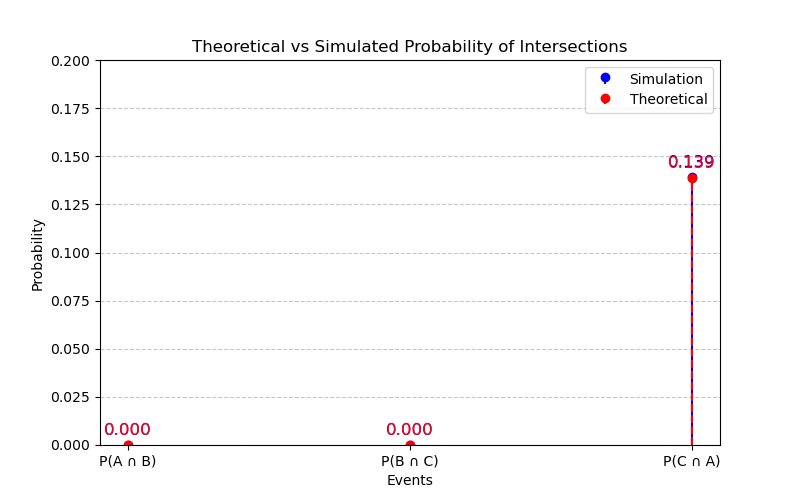
\includegraphics[width=\columnwidth]{figs/fig1.png}
    \caption{Theoritical vs Simulation}
    \label{fig:Plot1}
\end{figure}
}




\end{document}
